% Created by tikzDevice version 0.6.2-92-0ad2792 on 2013-03-11 01:35:44
% !TEX encoding = UTF-8 Unicode
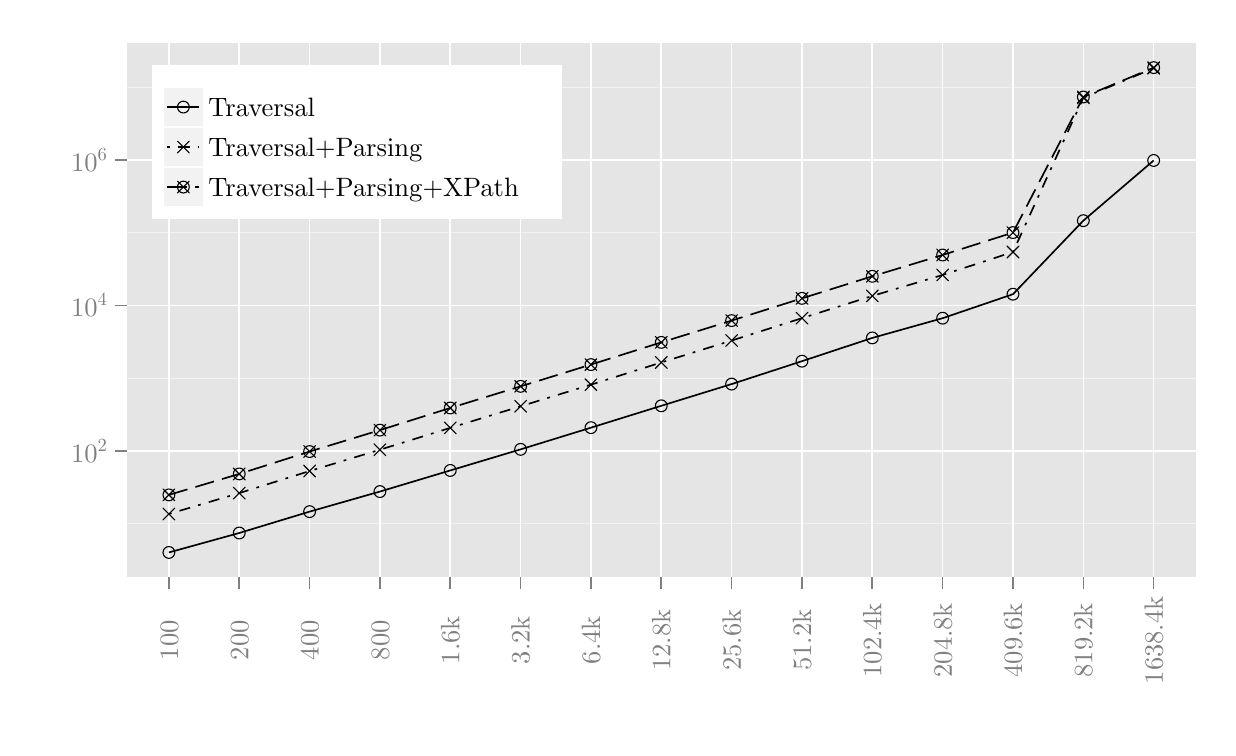
\begin{tikzpicture}[x=1pt,y=1pt]
\definecolor[named]{fillColor}{rgb}{1.00,1.00,1.00}
\path[use as bounding box,fill=fillColor,fill opacity=0.00] (0,0) rectangle (426.39,252.94);
\begin{scope}
\path[clip] (  0.00,  0.00) rectangle (426.39,252.94);
\definecolor[named]{drawColor}{rgb}{1.00,1.00,1.00}
\definecolor[named]{fillColor}{rgb}{1.00,1.00,1.00}

\path[draw=drawColor,line width= 0.6pt,line join=round,line cap=round,fill=fillColor] (  0.00,  0.00) rectangle (426.39,252.94);
\end{scope}
\begin{scope}
\path[clip] ( 35.78, 54.55) rectangle (422.13,247.25);
\definecolor[named]{fillColor}{rgb}{0.90,0.90,0.90}

\path[fill=fillColor] ( 35.78, 54.55) rectangle (422.13,247.25);
\definecolor[named]{drawColor}{rgb}{0.95,0.95,0.95}

\path[draw=drawColor,line width= 0.3pt,line join=round] ( 35.78, 73.82) --
	(422.13, 73.82);

\path[draw=drawColor,line width= 0.3pt,line join=round] ( 35.78,126.34) --
	(422.13,126.34);

\path[draw=drawColor,line width= 0.3pt,line join=round] ( 35.78,178.86) --
	(422.13,178.86);

\path[draw=drawColor,line width= 0.3pt,line join=round] ( 35.78,231.38) --
	(422.13,231.38);
\definecolor[named]{drawColor}{rgb}{1.00,1.00,1.00}

\path[draw=drawColor,line width= 0.6pt,line join=round] ( 35.78,100.08) --
	(422.13,100.08);

\path[draw=drawColor,line width= 0.6pt,line join=round] ( 35.78,152.60) --
	(422.13,152.60);

\path[draw=drawColor,line width= 0.6pt,line join=round] ( 35.78,205.12) --
	(422.13,205.12);

\path[draw=drawColor,line width= 0.6pt,line join=round] ( 51.03, 54.55) --
	( 51.03,247.25);

\path[draw=drawColor,line width= 0.6pt,line join=round] ( 76.45, 54.55) --
	( 76.45,247.25);

\path[draw=drawColor,line width= 0.6pt,line join=round] (101.87, 54.55) --
	(101.87,247.25);

\path[draw=drawColor,line width= 0.6pt,line join=round] (127.28, 54.55) --
	(127.28,247.25);

\path[draw=drawColor,line width= 0.6pt,line join=round] (152.70, 54.55) --
	(152.70,247.25);

\path[draw=drawColor,line width= 0.6pt,line join=round] (178.12, 54.55) --
	(178.12,247.25);

\path[draw=drawColor,line width= 0.6pt,line join=round] (203.54, 54.55) --
	(203.54,247.25);

\path[draw=drawColor,line width= 0.6pt,line join=round] (228.95, 54.55) --
	(228.95,247.25);

\path[draw=drawColor,line width= 0.6pt,line join=round] (254.37, 54.55) --
	(254.37,247.25);

\path[draw=drawColor,line width= 0.6pt,line join=round] (279.79, 54.55) --
	(279.79,247.25);

\path[draw=drawColor,line width= 0.6pt,line join=round] (305.20, 54.55) --
	(305.20,247.25);

\path[draw=drawColor,line width= 0.6pt,line join=round] (330.62, 54.55) --
	(330.62,247.25);

\path[draw=drawColor,line width= 0.6pt,line join=round] (356.04, 54.55) --
	(356.04,247.25);

\path[draw=drawColor,line width= 0.6pt,line join=round] (381.46, 54.55) --
	(381.46,247.25);

\path[draw=drawColor,line width= 0.6pt,line join=round] (406.87, 54.55) --
	(406.87,247.25);
\definecolor[named]{drawColor}{rgb}{0.00,0.00,0.00}

\path[draw=drawColor,line width= 0.6pt,line join=round] ( 51.03, 63.31) --
	( 76.45, 70.34) --
	(101.87, 78.06) --
	(127.28, 85.31) --
	(152.70, 92.94) --
	(178.12,100.56) --
	(203.54,108.40) --
	(228.95,116.30) --
	(254.37,124.15) --
	(279.79,132.42) --
	(305.20,140.83) --
	(330.62,147.96) --
	(356.04,156.63) --
	(381.46,183.20) --
	(406.87,204.95);

\path[draw=drawColor,line width= 0.6pt,dash pattern=on 1pt off 3pt on 4pt off 3pt ,line join=round] ( 51.03, 77.22) --
	( 76.45, 84.75) --
	(101.87, 92.73) --
	(127.28,100.43) --
	(152.70,108.32) --
	(178.12,116.12) --
	(203.54,123.94) --
	(228.95,131.96) --
	(254.37,139.88) --
	(279.79,147.97) --
	(305.20,156.00) --
	(330.62,163.58) --
	(356.04,171.87) --
	(381.46,227.61) --
	(406.87,238.28);

\path[draw=drawColor,line width= 0.6pt,dash pattern=on 7pt off 3pt ,line join=round] ( 51.03, 84.11) --
	( 76.45, 91.68) --
	(101.87, 99.77) --
	(127.28,107.51) --
	(152.70,115.51) --
	(178.12,123.33) --
	(203.54,131.20) --
	(228.95,139.22) --
	(254.37,147.09) --
	(279.79,155.13) --
	(305.20,163.10) --
	(330.62,170.79) --
	(356.04,178.89) --
	(381.46,227.89) --
	(406.87,238.50);

\path[draw=drawColor,line width= 0.4pt,line join=round,line cap=round] ( 51.03, 63.31) circle (  2.13);

\path[draw=drawColor,line width= 0.4pt,line join=round,line cap=round] ( 76.45, 70.34) circle (  2.13);

\path[draw=drawColor,line width= 0.4pt,line join=round,line cap=round] (101.87, 78.06) circle (  2.13);

\path[draw=drawColor,line width= 0.4pt,line join=round,line cap=round] (127.28, 85.31) circle (  2.13);

\path[draw=drawColor,line width= 0.4pt,line join=round,line cap=round] (152.70, 92.94) circle (  2.13);

\path[draw=drawColor,line width= 0.4pt,line join=round,line cap=round] (178.12,100.56) circle (  2.13);

\path[draw=drawColor,line width= 0.4pt,line join=round,line cap=round] (203.54,108.40) circle (  2.13);

\path[draw=drawColor,line width= 0.4pt,line join=round,line cap=round] (228.95,116.30) circle (  2.13);

\path[draw=drawColor,line width= 0.4pt,line join=round,line cap=round] (254.37,124.15) circle (  2.13);

\path[draw=drawColor,line width= 0.4pt,line join=round,line cap=round] (279.79,132.42) circle (  2.13);

\path[draw=drawColor,line width= 0.4pt,line join=round,line cap=round] (305.20,140.83) circle (  2.13);

\path[draw=drawColor,line width= 0.4pt,line join=round,line cap=round] (330.62,147.96) circle (  2.13);

\path[draw=drawColor,line width= 0.4pt,line join=round,line cap=round] (356.04,156.63) circle (  2.13);

\path[draw=drawColor,line width= 0.4pt,line join=round,line cap=round] (381.46,183.20) circle (  2.13);

\path[draw=drawColor,line width= 0.4pt,line join=round,line cap=round] (406.87,204.95) circle (  2.13);
\definecolor[named]{fillColor}{rgb}{1.00,1.00,1.00}

\path[draw=drawColor,line width= 0.4pt,line join=round,line cap=round,fill=fillColor] ( 48.90, 75.08) -- ( 53.16, 79.35);

\path[draw=drawColor,line width= 0.4pt,line join=round,line cap=round,fill=fillColor] ( 48.90, 79.35) -- ( 53.16, 75.08);

\path[draw=drawColor,line width= 0.4pt,line join=round,line cap=round,fill=fillColor] ( 74.31, 82.61) -- ( 78.58, 86.88);

\path[draw=drawColor,line width= 0.4pt,line join=round,line cap=round,fill=fillColor] ( 74.31, 86.88) -- ( 78.58, 82.61);

\path[draw=drawColor,line width= 0.4pt,line join=round,line cap=round,fill=fillColor] ( 99.73, 90.59) -- (104.00, 94.86);

\path[draw=drawColor,line width= 0.4pt,line join=round,line cap=round,fill=fillColor] ( 99.73, 94.86) -- (104.00, 90.59);

\path[draw=drawColor,line width= 0.4pt,line join=round,line cap=round,fill=fillColor] (125.15, 98.29) -- (129.42,102.56);

\path[draw=drawColor,line width= 0.4pt,line join=round,line cap=round,fill=fillColor] (125.15,102.56) -- (129.42, 98.29);

\path[draw=drawColor,line width= 0.4pt,line join=round,line cap=round,fill=fillColor] (150.57,106.18) -- (154.83,110.45);

\path[draw=drawColor,line width= 0.4pt,line join=round,line cap=round,fill=fillColor] (150.57,110.45) -- (154.83,106.18);

\path[draw=drawColor,line width= 0.4pt,line join=round,line cap=round,fill=fillColor] (175.98,113.99) -- (180.25,118.26);

\path[draw=drawColor,line width= 0.4pt,line join=round,line cap=round,fill=fillColor] (175.98,118.26) -- (180.25,113.99);

\path[draw=drawColor,line width= 0.4pt,line join=round,line cap=round,fill=fillColor] (201.40,121.80) -- (205.67,126.07);

\path[draw=drawColor,line width= 0.4pt,line join=round,line cap=round,fill=fillColor] (201.40,126.07) -- (205.67,121.80);

\path[draw=drawColor,line width= 0.4pt,line join=round,line cap=round,fill=fillColor] (226.82,129.82) -- (231.09,134.09);

\path[draw=drawColor,line width= 0.4pt,line join=round,line cap=round,fill=fillColor] (226.82,134.09) -- (231.09,129.82);

\path[draw=drawColor,line width= 0.4pt,line join=round,line cap=round,fill=fillColor] (252.24,137.75) -- (256.50,142.02);

\path[draw=drawColor,line width= 0.4pt,line join=round,line cap=round,fill=fillColor] (252.24,142.02) -- (256.50,137.75);

\path[draw=drawColor,line width= 0.4pt,line join=round,line cap=round,fill=fillColor] (277.65,145.84) -- (281.92,150.10);

\path[draw=drawColor,line width= 0.4pt,line join=round,line cap=round,fill=fillColor] (277.65,150.10) -- (281.92,145.84);

\path[draw=drawColor,line width= 0.4pt,line join=round,line cap=round,fill=fillColor] (303.07,153.87) -- (307.34,158.14);

\path[draw=drawColor,line width= 0.4pt,line join=round,line cap=round,fill=fillColor] (303.07,158.14) -- (307.34,153.87);

\path[draw=drawColor,line width= 0.4pt,line join=round,line cap=round,fill=fillColor] (328.49,161.45) -- (332.76,165.72);

\path[draw=drawColor,line width= 0.4pt,line join=round,line cap=round,fill=fillColor] (328.49,165.72) -- (332.76,161.45);

\path[draw=drawColor,line width= 0.4pt,line join=round,line cap=round,fill=fillColor] (353.91,169.74) -- (358.17,174.01);

\path[draw=drawColor,line width= 0.4pt,line join=round,line cap=round,fill=fillColor] (353.91,174.01) -- (358.17,169.74);

\path[draw=drawColor,line width= 0.4pt,line join=round,line cap=round,fill=fillColor] (379.32,225.47) -- (383.59,229.74);

\path[draw=drawColor,line width= 0.4pt,line join=round,line cap=round,fill=fillColor] (379.32,229.74) -- (383.59,225.47);

\path[draw=drawColor,line width= 0.4pt,line join=round,line cap=round,fill=fillColor] (404.74,236.15) -- (409.01,240.42);

\path[draw=drawColor,line width= 0.4pt,line join=round,line cap=round,fill=fillColor] (404.74,240.42) -- (409.01,236.15);

\path[draw=drawColor,line width= 0.4pt,line join=round,line cap=round] ( 51.03, 84.11) circle (  2.13);

\path[draw=drawColor,line width= 0.4pt,line join=round,line cap=round] ( 48.90, 81.98) -- ( 53.16, 86.25);

\path[draw=drawColor,line width= 0.4pt,line join=round,line cap=round] ( 48.90, 86.25) -- ( 53.16, 81.98);

\path[draw=drawColor,line width= 0.4pt,line join=round,line cap=round] ( 76.45, 91.68) circle (  2.13);

\path[draw=drawColor,line width= 0.4pt,line join=round,line cap=round] ( 74.31, 89.54) -- ( 78.58, 93.81);

\path[draw=drawColor,line width= 0.4pt,line join=round,line cap=round] ( 74.31, 93.81) -- ( 78.58, 89.54);

\path[draw=drawColor,line width= 0.4pt,line join=round,line cap=round] (101.87, 99.77) circle (  2.13);

\path[draw=drawColor,line width= 0.4pt,line join=round,line cap=round] ( 99.73, 97.64) -- (104.00,101.91);

\path[draw=drawColor,line width= 0.4pt,line join=round,line cap=round] ( 99.73,101.91) -- (104.00, 97.64);

\path[draw=drawColor,line width= 0.4pt,line join=round,line cap=round] (127.28,107.51) circle (  2.13);

\path[draw=drawColor,line width= 0.4pt,line join=round,line cap=round] (125.15,105.38) -- (129.42,109.64);

\path[draw=drawColor,line width= 0.4pt,line join=round,line cap=round] (125.15,109.64) -- (129.42,105.38);

\path[draw=drawColor,line width= 0.4pt,line join=round,line cap=round] (152.70,115.51) circle (  2.13);

\path[draw=drawColor,line width= 0.4pt,line join=round,line cap=round] (150.57,113.38) -- (154.83,117.64);

\path[draw=drawColor,line width= 0.4pt,line join=round,line cap=round] (150.57,117.64) -- (154.83,113.38);

\path[draw=drawColor,line width= 0.4pt,line join=round,line cap=round] (178.12,123.33) circle (  2.13);

\path[draw=drawColor,line width= 0.4pt,line join=round,line cap=round] (175.98,121.20) -- (180.25,125.47);

\path[draw=drawColor,line width= 0.4pt,line join=round,line cap=round] (175.98,125.47) -- (180.25,121.20);

\path[draw=drawColor,line width= 0.4pt,line join=round,line cap=round] (203.54,131.20) circle (  2.13);

\path[draw=drawColor,line width= 0.4pt,line join=round,line cap=round] (201.40,129.06) -- (205.67,133.33);

\path[draw=drawColor,line width= 0.4pt,line join=round,line cap=round] (201.40,133.33) -- (205.67,129.06);

\path[draw=drawColor,line width= 0.4pt,line join=round,line cap=round] (228.95,139.22) circle (  2.13);

\path[draw=drawColor,line width= 0.4pt,line join=round,line cap=round] (226.82,137.08) -- (231.09,141.35);

\path[draw=drawColor,line width= 0.4pt,line join=round,line cap=round] (226.82,141.35) -- (231.09,137.08);

\path[draw=drawColor,line width= 0.4pt,line join=round,line cap=round] (254.37,147.09) circle (  2.13);

\path[draw=drawColor,line width= 0.4pt,line join=round,line cap=round] (252.24,144.96) -- (256.50,149.23);

\path[draw=drawColor,line width= 0.4pt,line join=round,line cap=round] (252.24,149.23) -- (256.50,144.96);

\path[draw=drawColor,line width= 0.4pt,line join=round,line cap=round] (279.79,155.13) circle (  2.13);

\path[draw=drawColor,line width= 0.4pt,line join=round,line cap=round] (277.65,153.00) -- (281.92,157.26);

\path[draw=drawColor,line width= 0.4pt,line join=round,line cap=round] (277.65,157.26) -- (281.92,153.00);

\path[draw=drawColor,line width= 0.4pt,line join=round,line cap=round] (305.20,163.10) circle (  2.13);

\path[draw=drawColor,line width= 0.4pt,line join=round,line cap=round] (303.07,160.96) -- (307.34,165.23);

\path[draw=drawColor,line width= 0.4pt,line join=round,line cap=round] (303.07,165.23) -- (307.34,160.96);

\path[draw=drawColor,line width= 0.4pt,line join=round,line cap=round] (330.62,170.79) circle (  2.13);

\path[draw=drawColor,line width= 0.4pt,line join=round,line cap=round] (328.49,168.66) -- (332.76,172.93);

\path[draw=drawColor,line width= 0.4pt,line join=round,line cap=round] (328.49,172.93) -- (332.76,168.66);

\path[draw=drawColor,line width= 0.4pt,line join=round,line cap=round] (356.04,178.89) circle (  2.13);

\path[draw=drawColor,line width= 0.4pt,line join=round,line cap=round] (353.91,176.75) -- (358.17,181.02);

\path[draw=drawColor,line width= 0.4pt,line join=round,line cap=round] (353.91,181.02) -- (358.17,176.75);

\path[draw=drawColor,line width= 0.4pt,line join=round,line cap=round] (381.46,227.89) circle (  2.13);

\path[draw=drawColor,line width= 0.4pt,line join=round,line cap=round] (379.32,225.76) -- (383.59,230.02);

\path[draw=drawColor,line width= 0.4pt,line join=round,line cap=round] (379.32,230.02) -- (383.59,225.76);

\path[draw=drawColor,line width= 0.4pt,line join=round,line cap=round] (406.87,238.50) circle (  2.13);

\path[draw=drawColor,line width= 0.4pt,line join=round,line cap=round] (404.74,236.36) -- (409.01,240.63);

\path[draw=drawColor,line width= 0.4pt,line join=round,line cap=round] (404.74,240.63) -- (409.01,236.36);
\end{scope}
\begin{scope}
\path[clip] (  0.00,  0.00) rectangle (426.39,252.94);
\definecolor[named]{drawColor}{rgb}{0.50,0.50,0.50}

\node[text=drawColor,anchor=base west,inner sep=0pt, outer sep=0pt, scale=  0.96] at ( 15.71, 95.96) {10};

\node[text=drawColor,anchor=base west,inner sep=0pt, outer sep=0pt, scale=  0.67] at ( 25.31, 99.88) {2};

\node[text=drawColor,anchor=base west,inner sep=0pt, outer sep=0pt, scale=  0.96] at ( 15.71,148.48) {10};

\node[text=drawColor,anchor=base west,inner sep=0pt, outer sep=0pt, scale=  0.67] at ( 25.31,152.40) {4};

\node[text=drawColor,anchor=base west,inner sep=0pt, outer sep=0pt, scale=  0.96] at ( 15.71,201.00) {10};

\node[text=drawColor,anchor=base west,inner sep=0pt, outer sep=0pt, scale=  0.67] at ( 25.31,204.93) {6};
\end{scope}
\begin{scope}
\path[clip] (  0.00,  0.00) rectangle (426.39,252.94);
\definecolor[named]{drawColor}{rgb}{0.50,0.50,0.50}

\path[draw=drawColor,line width= 0.6pt,line join=round] ( 31.51,100.08) --
	( 35.78,100.08);

\path[draw=drawColor,line width= 0.6pt,line join=round] ( 31.51,152.60) --
	( 35.78,152.60);

\path[draw=drawColor,line width= 0.6pt,line join=round] ( 31.51,205.12) --
	( 35.78,205.12);
\end{scope}
\begin{scope}
\path[clip] (  0.00,  0.00) rectangle (426.39,252.94);
\definecolor[named]{drawColor}{rgb}{0.50,0.50,0.50}

\path[draw=drawColor,line width= 0.6pt,line join=round] ( 51.03, 50.28) --
	( 51.03, 54.55);

\path[draw=drawColor,line width= 0.6pt,line join=round] ( 76.45, 50.28) --
	( 76.45, 54.55);

\path[draw=drawColor,line width= 0.6pt,line join=round] (101.87, 50.28) --
	(101.87, 54.55);

\path[draw=drawColor,line width= 0.6pt,line join=round] (127.28, 50.28) --
	(127.28, 54.55);

\path[draw=drawColor,line width= 0.6pt,line join=round] (152.70, 50.28) --
	(152.70, 54.55);

\path[draw=drawColor,line width= 0.6pt,line join=round] (178.12, 50.28) --
	(178.12, 54.55);

\path[draw=drawColor,line width= 0.6pt,line join=round] (203.54, 50.28) --
	(203.54, 54.55);

\path[draw=drawColor,line width= 0.6pt,line join=round] (228.95, 50.28) --
	(228.95, 54.55);

\path[draw=drawColor,line width= 0.6pt,line join=round] (254.37, 50.28) --
	(254.37, 54.55);

\path[draw=drawColor,line width= 0.6pt,line join=round] (279.79, 50.28) --
	(279.79, 54.55);

\path[draw=drawColor,line width= 0.6pt,line join=round] (305.20, 50.28) --
	(305.20, 54.55);

\path[draw=drawColor,line width= 0.6pt,line join=round] (330.62, 50.28) --
	(330.62, 54.55);

\path[draw=drawColor,line width= 0.6pt,line join=round] (356.04, 50.28) --
	(356.04, 54.55);

\path[draw=drawColor,line width= 0.6pt,line join=round] (381.46, 50.28) --
	(381.46, 54.55);

\path[draw=drawColor,line width= 0.6pt,line join=round] (406.87, 50.28) --
	(406.87, 54.55);
\end{scope}
\begin{scope}
\path[clip] (  0.00,  0.00) rectangle (426.39,252.94);
\definecolor[named]{drawColor}{rgb}{0.50,0.50,0.50}

\node[text=drawColor,rotate= 90.00,anchor=base,inner sep=0pt, outer sep=0pt, scale=  0.96] at ( 54.34, 31.57) {100};

\node[text=drawColor,rotate= 90.00,anchor=base,inner sep=0pt, outer sep=0pt, scale=  0.96] at ( 79.75, 31.57) {200};

\node[text=drawColor,rotate= 90.00,anchor=base,inner sep=0pt, outer sep=0pt, scale=  0.96] at (105.17, 31.57) {400};

\node[text=drawColor,rotate= 90.00,anchor=base,inner sep=0pt, outer sep=0pt, scale=  0.96] at (130.59, 31.57) {800};

\node[text=drawColor,rotate= 90.00,anchor=base,inner sep=0pt, outer sep=0pt, scale=  0.96] at (156.01, 31.57) {1.6k};

\node[text=drawColor,rotate= 90.00,anchor=base,inner sep=0pt, outer sep=0pt, scale=  0.96] at (181.42, 31.57) {3.2k};

\node[text=drawColor,rotate= 90.00,anchor=base,inner sep=0pt, outer sep=0pt, scale=  0.96] at (206.84, 31.57) {6.4k};

\node[text=drawColor,rotate= 90.00,anchor=base,inner sep=0pt, outer sep=0pt, scale=  0.96] at (232.26, 31.57) {12.8k};

\node[text=drawColor,rotate= 90.00,anchor=base,inner sep=0pt, outer sep=0pt, scale=  0.96] at (257.68, 31.57) {25.6k};

\node[text=drawColor,rotate= 90.00,anchor=base,inner sep=0pt, outer sep=0pt, scale=  0.96] at (283.09, 31.57) {51.2k};

\node[text=drawColor,rotate= 90.00,anchor=base,inner sep=0pt, outer sep=0pt, scale=  0.96] at (308.51, 31.57) {102.4k};

\node[text=drawColor,rotate= 90.00,anchor=base,inner sep=0pt, outer sep=0pt, scale=  0.96] at (333.93, 31.57) {204.8k};

\node[text=drawColor,rotate= 90.00,anchor=base,inner sep=0pt, outer sep=0pt, scale=  0.96] at (359.35, 31.57) {409.6k};

\node[text=drawColor,rotate= 90.00,anchor=base,inner sep=0pt, outer sep=0pt, scale=  0.96] at (384.76, 31.57) {819.2k};

\node[text=drawColor,rotate= 90.00,anchor=base,inner sep=0pt, outer sep=0pt, scale=  0.96] at (410.18, 31.57) {1638.4k};
\end{scope}
\begin{scope}
\path[clip] (  0.00,  0.00) rectangle (426.39,252.94);
\definecolor[named]{fillColor}{rgb}{1.00,1.00,1.00}

\path[fill=fillColor] ( 44.77,183.85) rectangle (192.92,239.36);
\end{scope}
\begin{scope}
\path[clip] (  0.00,  0.00) rectangle (426.39,252.94);
\definecolor[named]{drawColor}{rgb}{1.00,1.00,1.00}
\definecolor[named]{fillColor}{rgb}{0.95,0.95,0.95}

\path[draw=drawColor,line width= 0.6pt,line join=round,line cap=round,fill=fillColor] ( 49.03,217.02) rectangle ( 63.49,231.48);
\end{scope}
\begin{scope}
\path[clip] (  0.00,  0.00) rectangle (426.39,252.94);
\definecolor[named]{drawColor}{rgb}{0.00,0.00,0.00}

\path[draw=drawColor,line width= 0.6pt,line join=round] ( 50.48,224.25) -- ( 62.04,224.25);
\end{scope}
\begin{scope}
\path[clip] (  0.00,  0.00) rectangle (426.39,252.94);
\definecolor[named]{drawColor}{rgb}{0.00,0.00,0.00}

\path[draw=drawColor,line width= 0.4pt,line join=round,line cap=round] ( 56.26,224.25) circle (  2.13);
\end{scope}
\begin{scope}
\path[clip] (  0.00,  0.00) rectangle (426.39,252.94);
\definecolor[named]{drawColor}{rgb}{1.00,1.00,1.00}
\definecolor[named]{fillColor}{rgb}{0.95,0.95,0.95}

\path[draw=drawColor,line width= 0.6pt,line join=round,line cap=round,fill=fillColor] ( 49.03,202.57) rectangle ( 63.49,217.02);
\end{scope}
\begin{scope}
\path[clip] (  0.00,  0.00) rectangle (426.39,252.94);
\definecolor[named]{drawColor}{rgb}{0.00,0.00,0.00}

\path[draw=drawColor,line width= 0.6pt,dash pattern=on 1pt off 3pt on 4pt off 3pt ,line join=round] ( 50.48,209.80) -- ( 62.04,209.80);
\end{scope}
\begin{scope}
\path[clip] (  0.00,  0.00) rectangle (426.39,252.94);
\definecolor[named]{drawColor}{rgb}{0.00,0.00,0.00}
\definecolor[named]{fillColor}{rgb}{1.00,1.00,1.00}

\path[draw=drawColor,line width= 0.4pt,line join=round,line cap=round,fill=fillColor] ( 54.13,207.66) -- ( 58.40,211.93);

\path[draw=drawColor,line width= 0.4pt,line join=round,line cap=round,fill=fillColor] ( 54.13,211.93) -- ( 58.40,207.66);
\end{scope}
\begin{scope}
\path[clip] (  0.00,  0.00) rectangle (426.39,252.94);
\definecolor[named]{drawColor}{rgb}{1.00,1.00,1.00}
\definecolor[named]{fillColor}{rgb}{0.95,0.95,0.95}

\path[draw=drawColor,line width= 0.6pt,line join=round,line cap=round,fill=fillColor] ( 49.03,188.12) rectangle ( 63.49,202.57);
\end{scope}
\begin{scope}
\path[clip] (  0.00,  0.00) rectangle (426.39,252.94);
\definecolor[named]{drawColor}{rgb}{0.00,0.00,0.00}

\path[draw=drawColor,line width= 0.6pt,dash pattern=on 7pt off 3pt ,line join=round] ( 50.48,195.34) -- ( 62.04,195.34);
\end{scope}
\begin{scope}
\path[clip] (  0.00,  0.00) rectangle (426.39,252.94);
\definecolor[named]{drawColor}{rgb}{0.00,0.00,0.00}

\path[draw=drawColor,line width= 0.4pt,line join=round,line cap=round] ( 56.26,195.34) circle (  2.13);

\path[draw=drawColor,line width= 0.4pt,line join=round,line cap=round] ( 54.13,193.21) -- ( 58.40,197.48);

\path[draw=drawColor,line width= 0.4pt,line join=round,line cap=round] ( 54.13,197.48) -- ( 58.40,193.21);
\end{scope}
\begin{scope}
\path[clip] (  0.00,  0.00) rectangle (426.39,252.94);
\definecolor[named]{drawColor}{rgb}{0.00,0.00,0.00}

\node[text=drawColor,anchor=base west,inner sep=0pt, outer sep=0pt, scale=  0.96] at ( 65.29,220.95) {Traversal $\;\;\;$};
\end{scope}
\begin{scope}
\path[clip] (  0.00,  0.00) rectangle (426.39,252.94);
\definecolor[named]{drawColor}{rgb}{0.00,0.00,0.00}

\node[text=drawColor,anchor=base west,inner sep=0pt, outer sep=0pt, scale=  0.96] at ( 65.29,206.49) {Traversal+Parsing $\;\;\;$};
\end{scope}
\begin{scope}
\path[clip] (  0.00,  0.00) rectangle (426.39,252.94);
\definecolor[named]{drawColor}{rgb}{0.00,0.00,0.00}

\node[text=drawColor,anchor=base west,inner sep=0pt, outer sep=0pt, scale=  0.96] at ( 65.29,192.04) {Traversal+Parsing+XPath $\;\;\;$};
\end{scope}
\end{tikzpicture}
